\documentclass{beamer}

\usepackage[T1]{fontenc}
\usepackage[polish]{babel}
\usepackage[utf8]{inputenc}
\usepackage{lmodern}
\usepackage{amsmath}

\selectlanguage{polish}

\mode<presentation> {
	\usetheme{Copenhagen}
}

\usepackage{graphicx} % Allows including images
\usepackage{booktabs} % Allows the use of \toprule, \midrule and \bottomrule in tables

\newcommand{\red}[1]{
	{ \color{red}{#1} }
}

\newcommand{\score}[2]{
	\stackrel
	{\red{#1}}
	{#2}
}

\definecolor{links}{HTML}{2A1B81}
\hypersetup{colorlinks,linkcolor=,urlcolor=links}

%----------------------------------------------------------------------------------------
%	TITLE PAGE
%----------------------------------------------------------------------------------------

\title
[System obliczający wyniki wyborów]
{Studium wykonalności i aktualny stan prac}

\author
[T. Kasprzyk, D. Ogiela, J. Stępak]
{Tomasz Kasprzyk, \ Daniel Ogiela, \ Jakub Stępak}

\institute
[AGH]
{
Akademia Górniczo-Hutnicza

Wydział Informatyki, Elektroniki i Telekomunikacji

Katedra Informatyki 

}
\date{9 maja 2016}

\begin{document}

\frame{\titlepage}

\begin{frame}
\frametitle{Plan prezentacji}
\tableofcontents
\end{frame}

%----------------------------------------------------------------------------------------
%	PRESENTATION SLIDES
%----------------------------------------------------------------------------------------

%------------------------------------------------
\section{Studium wykonalności}
%------------------------------------------------
\subsection{Wymagania wobec produktu końcowego}

\begin{frame}

\frametitle{Zadania produktu końcowego}
\begin{itemize}
\item Poprawne obliczanie wyników wyborów w zadanym systemie wyborczym
\item Obliczanie wyników wyborów w możliwie najkrótszym czasie
\item Przystępna dla użytkownika prezentacja wyników wyborów
\end{itemize}

\end{frame}

\begin{frame}

\frametitle{Sposób działania produktu końcowego}
\begin{itemize}
\item Aplikacja internetowa umożliwiająca zdefiniowanie wyborów
\item Zdefiniowanie wyborów ma polegać na określeniu kandydatów, preferencji głosujących i rozmiaru zwycięskiego komitetu
\item Użytkownik posiada różne sposoby zdefiniowania wyborów:
\begin{enumerate}
\item Wczytanie pliku w odpowiednim formacie (.soc)
\item Generacja z rozkładu normalnego
\item Graficzna generacja preferencji wyborców
\end{enumerate}
\item System oblicza wyniki wyborów dla określonych przez użytkownika wartości parametru p
\end{itemize}

\end{frame}

% ---------------------------------------------------
\subsection{Strategia testowania}

\begin{frame}

\frametitle{Rodzaje pisanych testów}
\begin{itemize}
\item Testy jednostkowe do sprawdzenia poprawności działania kolejnych komponentów projektu
\item Testy regresywne do sprawdzenia poprawności działania wcześniej dodanych elementów systemu po dodaniu nowych elementów
\item Testy porównawcze do sprawdzenia skuteczności obliczania wyników wyborów
\end{itemize}

\end{frame}

\begin{frame}

\frametitle{Ocena poprawności działania produktu}
\begin{itemize}
\item Testy porównawcze głównego algorytmu obliczającego wyniki wyborów z algorytmami innego typu
\item Dla mniejszego rozmiaru danych wejściowych porównanie działania z algorytmem typu brute-force
\item Dla większego rozmiaru danych wejściowych porównanie działania z innym algorytmem heurystycznym np. algorytmem zachłannym
\end{itemize}

\end{frame}

%---------------------------------------------------
\subsection{Aspekt technologiczny}

\begin{frame}

\frametitle{Wykorzystane technologie}
\begin{itemize}
\item Python 2.7
\item Django 1.9
\item Bootstrap
\item JavaScipt (jQuery i Chart.js)
\item Platforma Heroku do wdrożenia systemu
\item Ciągła integracja: Travis + Coveralls
\end{itemize}

\end{frame}

\begin{frame}

\frametitle{Wybór technologii}
\begin{itemize}
\item Doświadczenie części zespołu w pracy z wybraną technologią
\item Przekonanie o możliwości zrealizowania projektu w wybranej technologii
\item Zaoszczędzenie czasu na poznawanie nowych technologii
\item Wydajność
\end{itemize}

\end{frame}

% ----------------------------------------------------

\subsection{Plan}

\begin{frame}

\frametitle{Szansa na powodzenie i przewidzenie trudności}
\begin{itemize}
\item Przekonanie o możliwości zrealizowania harmonogramu prac określonego w wizji i wykonania produktu na czas
\item Główne problemy przewidywane przy projektowaniu i implementacji głównego algorytmu obliczającego wyniki wyborów – algorytmu genetycznego
\item Zwiększone nakłady pracy całego zespołu w przypadku napotkania trudności i skupienie całego wysiłku na tym zadaniu
\end{itemize}

\end{frame}

% ----------------------------------------------------

\section{Aktualny stan prac}

\subsection{Zrealizowane zadania}

\begin{frame}

\frametitle{Co już jest}
\begin{itemize}
\item Implementacja algorytmu brute-force
\item Generacja wyborów z rozkładu normalnego
\item Wczytywanie wyborów z pliku wraz z ich walidacją
\item Webowy interface
\item Tworzenie wykresów 2D
\item Konfiguracja wdrożenia systemu na Heroku
\end{itemize}

\end{frame}


\begin{frame}
\frametitle{Gdzie zobaczyć nasz produkt}

\begin{itemize}
\item Adres repozytorium: \linebreak
	\url{https://github.com/jakubste/election-computing-system}
\item Działająca aplikacja: 
	\url{https://election-computing-system.herokuapp.com}
\end{itemize}

\end{frame}


\begin{frame}
\hspace*{-1.1cm}
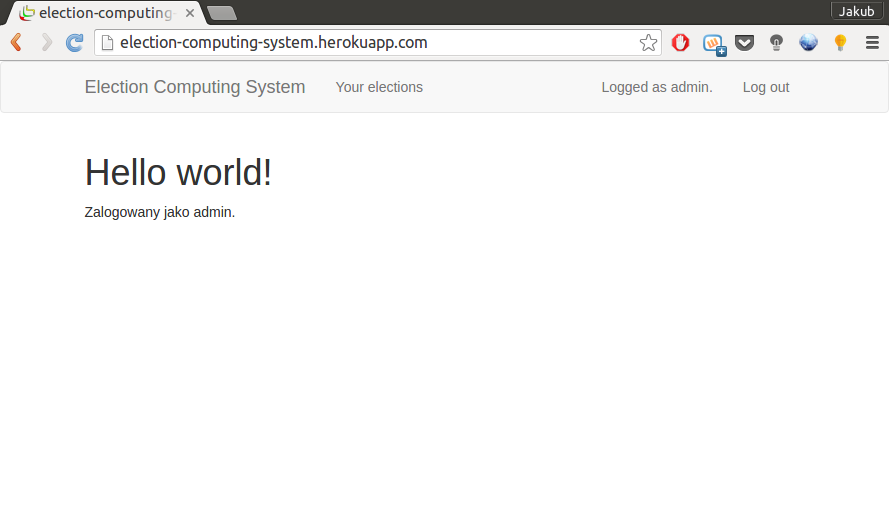
\includegraphics[width=\paperwidth]{screenshots/main_page}
\end{frame}

\begin{frame}
\hspace*{-1.1cm}
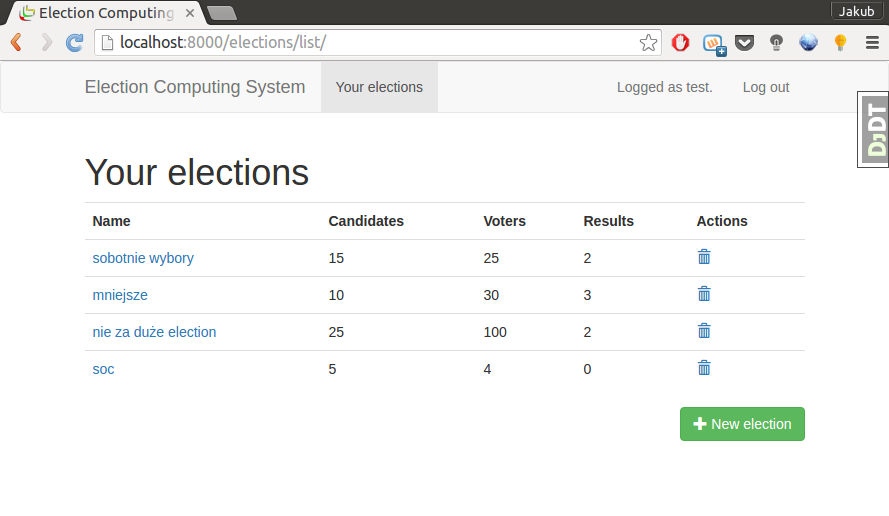
\includegraphics[width=\paperwidth]{screenshots/election_list}
\end{frame}

\begin{frame}
\begin{center}
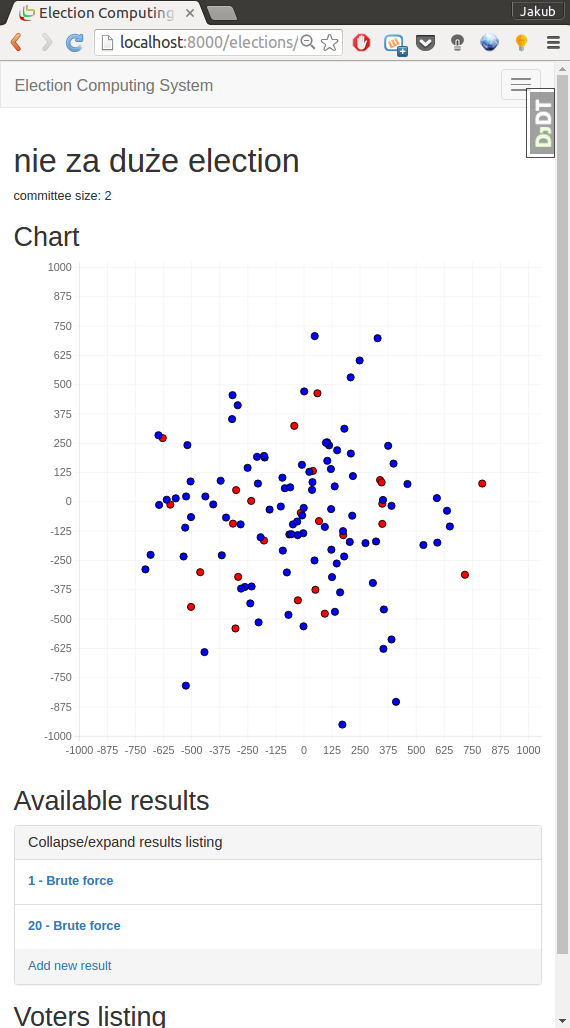
\includegraphics[height=\paperheight]{screenshots/election_details}
\end{center}
\end{frame}

\begin{frame}
\begin{center}
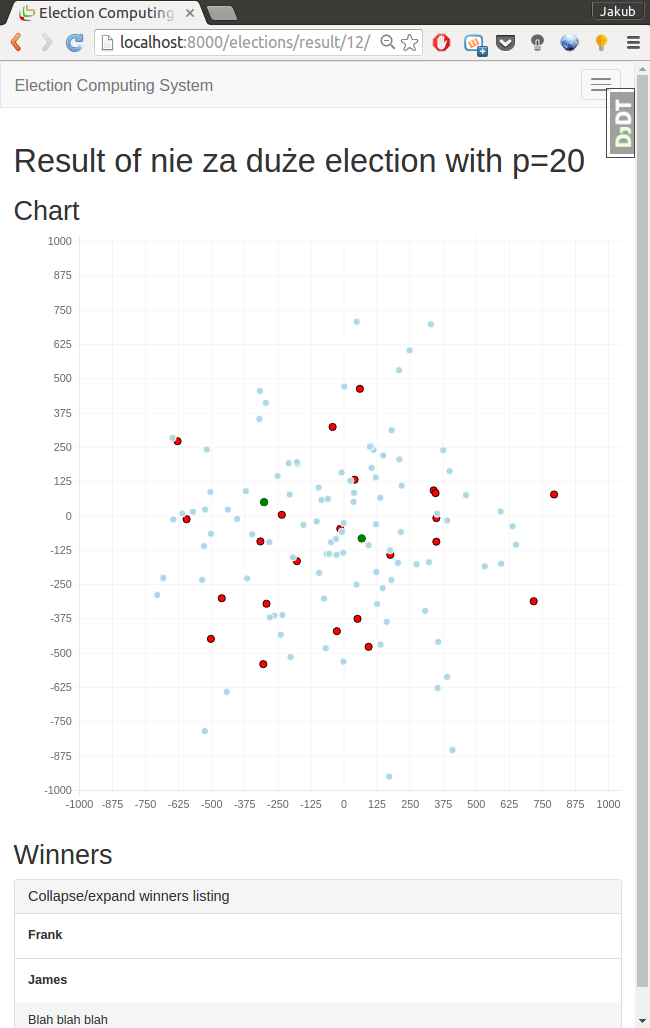
\includegraphics[height=\paperheight]{screenshots/election_results}
\end{center}
\end{frame}


% ----------------------------------------------------

\subsection{Zadania do zrealizowania na najbliższe tygodnie}

\begin{frame}

\frametitle{Co do zrobienia}
\begin{itemize}
\item Algorytm zachłanny do obliczania wyników wyborów	
\item Algorytm genetyczny do obliczania wyników wyborów
\item Polepszenie interfejsu i UX
\end{itemize}

\end{frame}


% ----------------------------------------------------


\begin{frame}
\Huge{\centerline{Dziękujemy za uwagę}}
\end{frame}

\end{document}